\section{Development}
\subsection{flashing the Texas Instrument Sensor-Tag}
In order to flash the sensor tag, SmartRF Flash Programmer 2 made by Texas Instrument has been used. For flashing the node a sensor tag needs a Debugger DevPack, the debugger allow to communicate to the sensor via USB as it is shown in the picture \ref{fig:debugger}. The 
\begin{figure}[!h]
	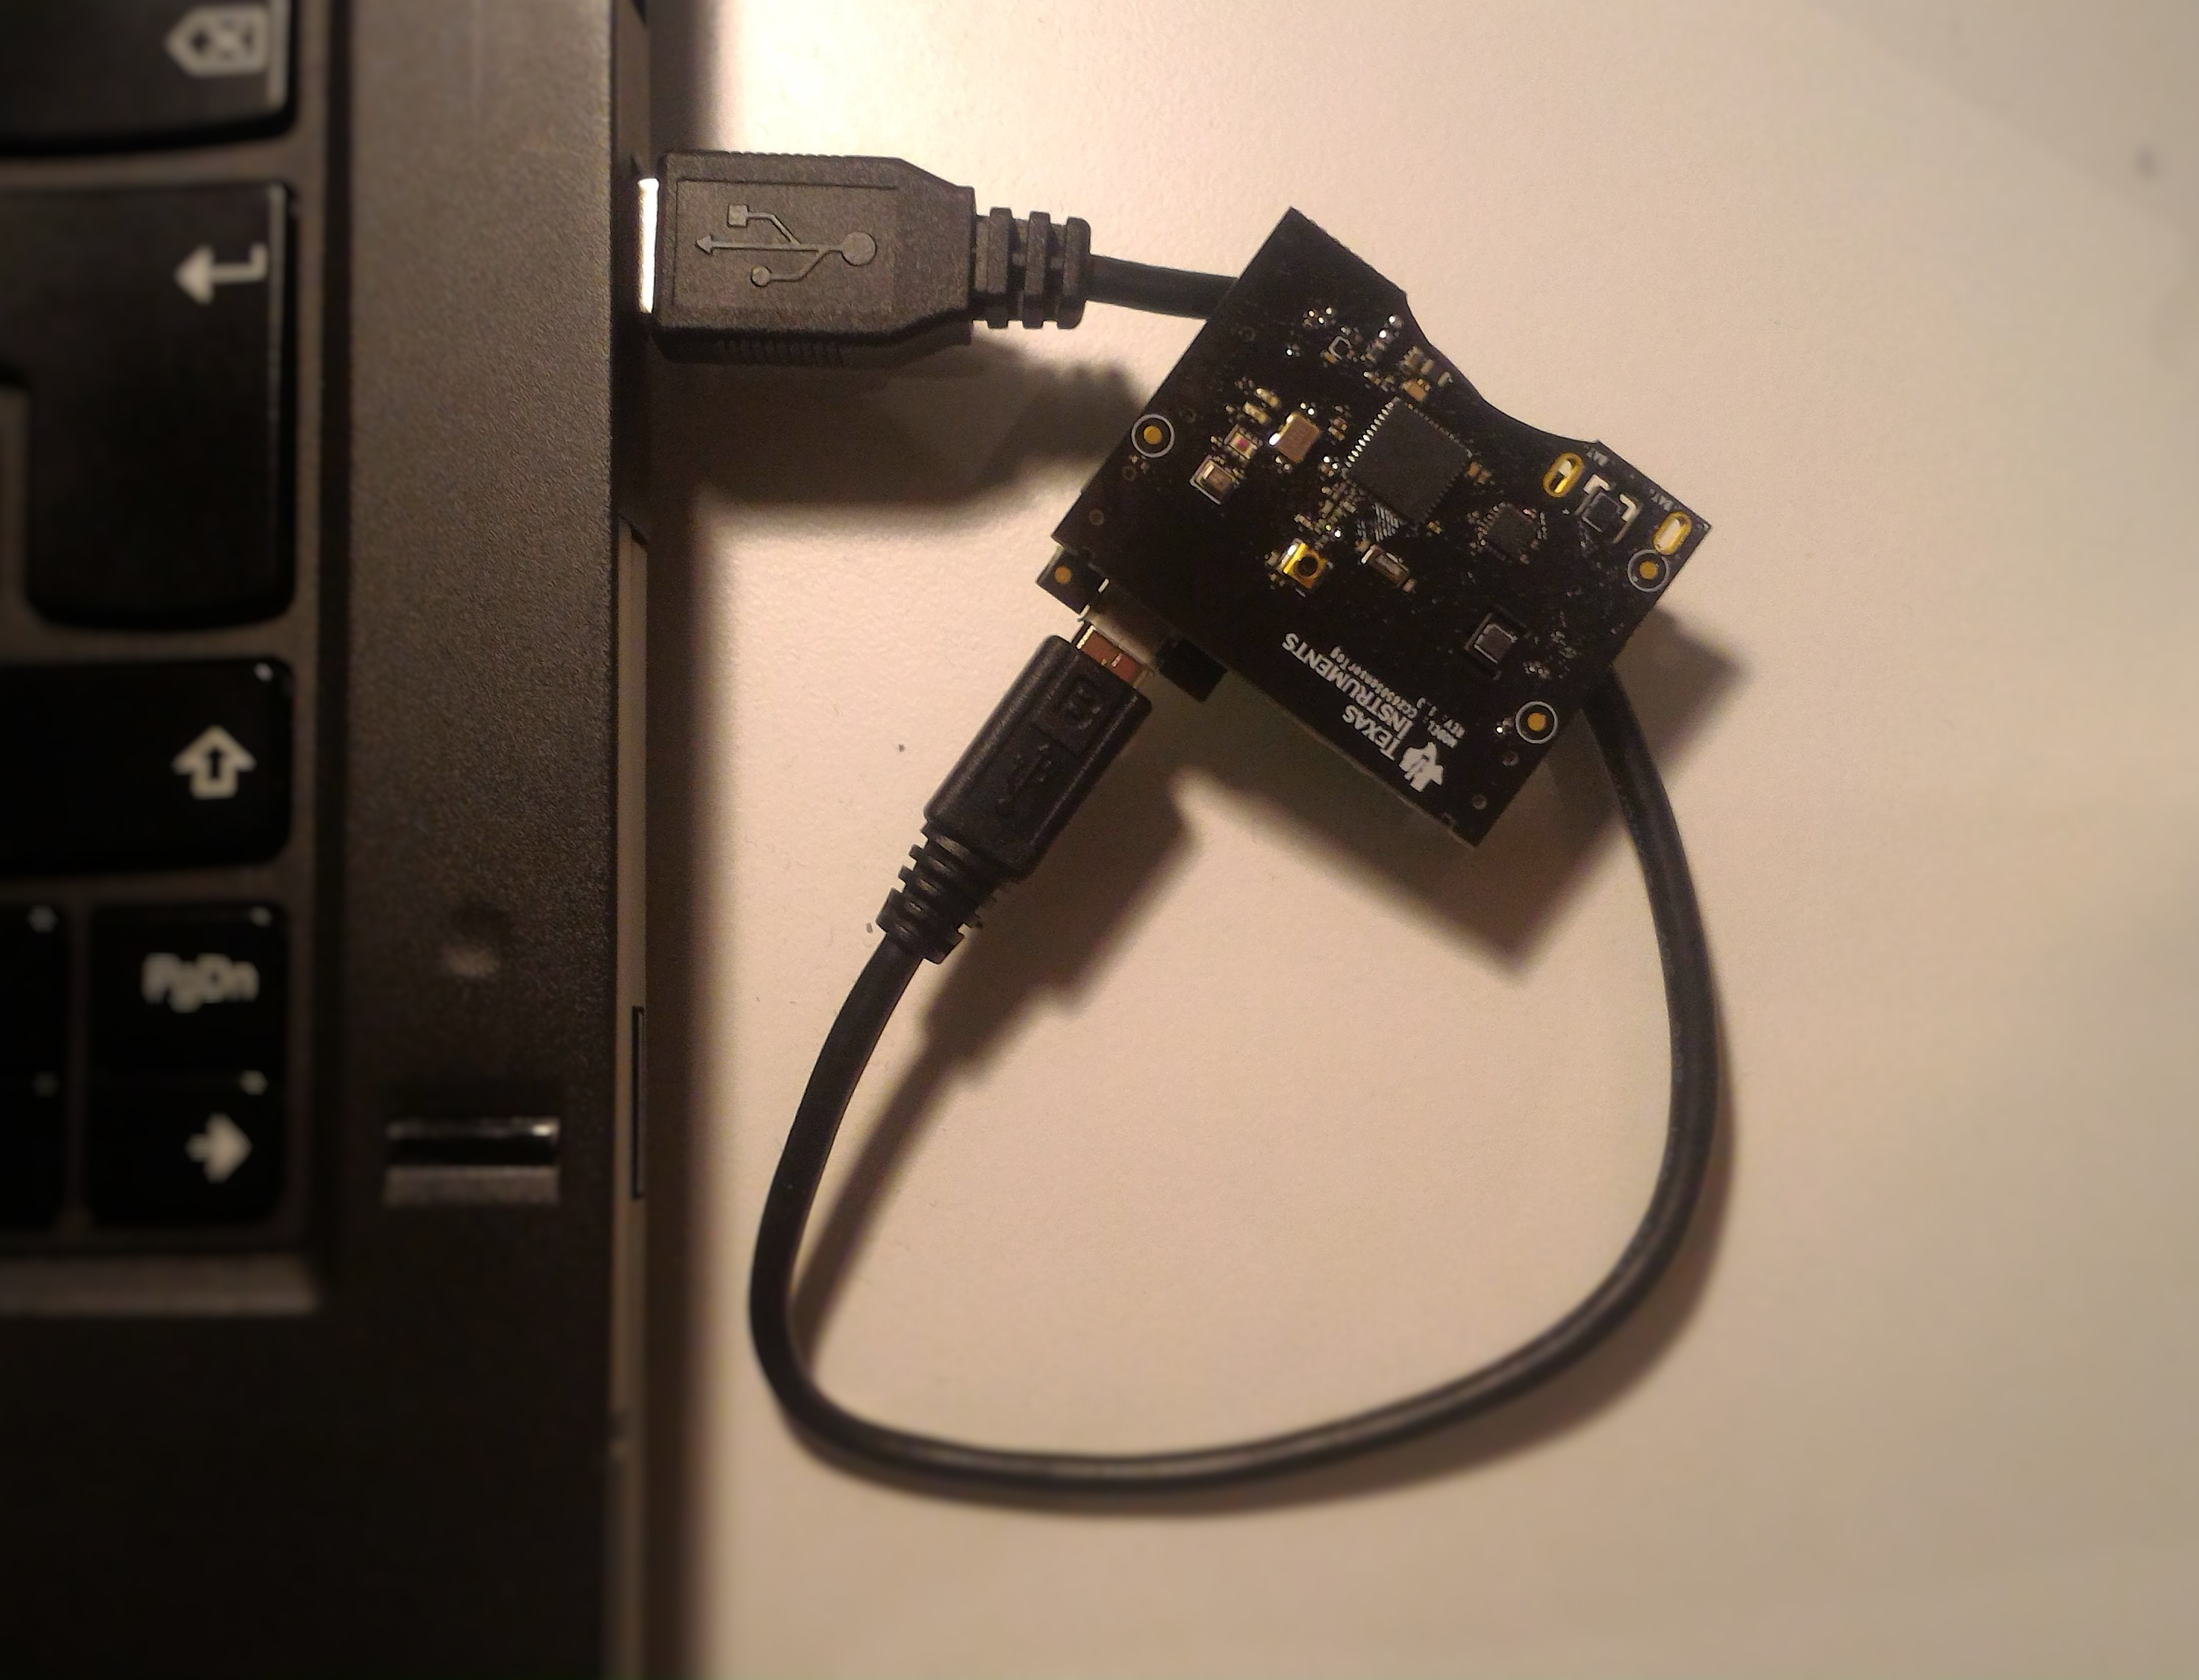
\includegraphics[width=\linewidth]{debugger}
	\caption{sensor node connected with the debugger to a computer}
	\label{fig:debugger}
\end{figure} 

\subsection{title}